\chapter{Paper:~Low TPA and free-carrier effects in Si-nanocrystal slot}
\label{ch:articleTimeRes}
\pagestyle{plain}

In the previous chapter, ultrafast Si-nanocrystal-based optical logic gates were demonstrated. However, a proper quantification of the carrier effects and TPA was missing. In order to characterize separately all these nonlinear effects, we set up an advanced experiment capable of measuring the ultrafast nonlinear response in phase and amplitude. We performed measurements on a Si-nanocrystal slot sample and compared it to standard Si strip waveguides, where we were able to quantitatively conclude the better performance of the silicon-nanocrystal slot through its nonlinear figure-of-merit.

The paper was the result of a collaboration between my group in UPV, the group of Dr. I. Cristiani, in Uniersity of Pavia, and CEA LETI in Grenoble, France, who fabricated the samples. My personal contribution to the work is the following: I made the experimental measurements, together with C. Lacava; I analyzed the data and drafted the paper. Simulations of the waveguides were done by Guillem Ballesteros and Paolo Minzioni independently, reaching the same results. The paper was published in Optics Express, and the reference is the following:

\vspace{1.5cm}

J Matres, C Lacava, G C Ballesteros, P Minzioni, I Cristiani, J Marti, J M Fedeli, and C J Oton. Low TPA and free-carrier effects in silicon nanocrystal-based horizontal slot waveguides. Opt. Express, 20(21):23838–23845, October 2012

\newpage
\begin{center}
\section*{Low TPA and free-carrier effects in silicon nanocrystal-based horizontal slot waveguides}
{J. Matres,$^{*,1}$ C. Lacava,$^2$ G. C. Ballesteros,$^1$ P. Minzioni,$^2$ I. Cristiani,$^2$ J.~M.~F\'ed\'eli,$^3$ J. Mart\'i,$^1$ and C. J. Oton,$^1$} 
\end{center}
\noindent
\textit{$^1$ Nanophotonics Technology Center, Universidad Polit\'ecnica de Valencia, Camino de Vera s/n, 46022, Valencia, Spain\\
$^2$Dipartimento di Ingegneria Industriale e dell'Informazione, Universita di Pavia, Via Ferrata 1, 27100, Pavia, Italy\\
$^3$CEA LETI, Minatec Campus, Grenoble 38054, France}

\begin{center}
{$^*$joamatab@ntc.upv.es}

%%%%%%%%%%%%%%%%%%% abstract and OCIS codes %%%%%%%%%%%%%%%%
%% [use \begin{abstract*}...\end{abstract*} if exempt from copyright]

\end{center}


%\begin{abstract}
\textbf{Abstract} \\
\noindent
We present the characterization of the ultrafast nonlinear dynamics of a CMOS-compatible horizontal-slot waveguide with silicon nanocrystals.
Results are compared to strip silicon waveguides, and modeled with nonlinear split-step calculations.
The extracted parameters show that the slot waveguide has weaker carrier effects and better nonlinear figure-of-merit than the strip waveguides. 
%\end{abstract}

\begin{center}
{(190.0190) Nonlinear optics; (130.0130) Integrated optics; (320.0320) Ultrafast optics; (160.4330) Nonlinear optical materials.}
\end{center}
%(220.0220) Optical design and fabrication; (230.5750) Resonators; (230.3990) Microstructure devices; (250.5300) Photonic Integrated Circuits.}

%%%%%%%%%%%%%%%%%%%%%%% References %%%%%%%%%%%%%%%%%%%%%%%%%



\section{Introduction}
Nonlinear silicon-based photonic devices can introduce key functionalities for on-chip optical signal processing and routing. In the last years, many different nonlinear silicon devices have been reported, such as all-optical modulators~\cite{Almeida2004b}, wavelength converters~\cite{Lee2009,Driscoll2010}, demultiplexers~\cite{Koos2009}, format converters~\cite{Astar2010}, etc.
These nonlinear devices can be based either on free carriers or on the bound-electron Kerr coefficient.
In pure silicon waveguides, the Kerr effect is usually hindered by more intense and longer-lasting free-carrier dispersion (FCD)~\cite{Foster2008,Osgood2009}. However, it is often desirable to exploit the Kerr effect, as its temporal response is instantaneous (thus allowing high-speed operation) and it enables parametric conversion and amplification. In order to increase the Kerr coefficient and reduce carrier effects in silicon waveguides, a slot-type geometry~\cite{Almeida2004} was proposed~\cite{Sanchis2007,Koos2007a,Zhang2010,Rukhlenko2012}, where a thin layer of a low-index material material with high nonlinear coefficient is sandwiched between two silicon channels.
A vertical slot geometry was also demonstrated to allow the introduction of an organic polymer, and this device showed optical 160~Gb/s demultiplexing capabilities~\cite{Koos2009}; however, these materials involve non-CMOS processes and impose strict temperature limitations.
On the other hand, silicon-nanocrystal-based horizontal slot waveguides only require CMOS processes, and have recently demonstrated ultrafast all-optical modulation capabilities and good nonlinear properties~\cite{Spano2009, Martinez2010a, Oton2010, Trita2011}.
In this paper, we study the nonlinear ultrafast dynamics of this type of waveguide, where we show that the effect of carriers is greatly reduced as compared to silicon channel waveguides. We also report quantitative measurements of nonlinear absorption of these waveguides.
Finally we show simulation results which fit the experimental data and provide estimations of the nonlinear parameters and figures of merit of the waveguides.


\section{Fabrication}
Slot samples were fabricated starting from silicon--on--insulator (SOI) wafers with 220~nm Si thickness.
On top of the Si layer, a 100~nm--thick layer of silicon--rich silica ($ \mathrm{SiO_x} $) was grown by plasma-enhanced chemical vapor deposition (PECVD) using a gas ratio of $[N_2O/SiH_4]=180/20$ subsequently annealed at $1000^\circ$ ~in $ \mathrm{N}_2 $ ambient for 210~s.
The nominal amount of silicon excess was 16\% and Silicon-nanocrystals had an average size of 4~nm.
The value of Si-excess was determined by using the X-ray photoelectron spectroscopy (XPS) and the average size of formed Si-nc was determined by means of the Energy Filtered Transmission Electron Microscopy EFTEM. Both these techniques are well described in~\cite{Garcia2004}.
The top layer of the slot structure was fabricated using an hydrogenated amorphous silicon layer.
Annealing temperature was set to $400^\circ$ C to avoid the silicon crystallization process.
The nano-slot fabrication process was previously optimized in order to obtain a low-loss and high nonlinear performance as described in~\cite{Jordana2007}.
Waveguides were patterned with deep-UV lithography and etched down to the buried oxide to form channels as the ones reported in~\cite{Martinez2010a, Trita2011}.
The whole layout was covered with silica after the etching process as shown in Fig.~\ref{fig:semSlot}.
On the other hand, two Si strip waveguides were fabricated for comparison, always starting  from SOI wafers patterned with deep-UV lithography.
Their dimensions were $445\times220$~nm for transverse-electric (TE) polarization and $485\times220$~nm for transverse-magnetic (TM) polarization, both with a length of 25~mm.
The slot waveguide, where the TM-polarized mode was excited to exploit the E-field magnification effect in the slot region, was 7~mm long.


\begin{figure}[htb]
\centering
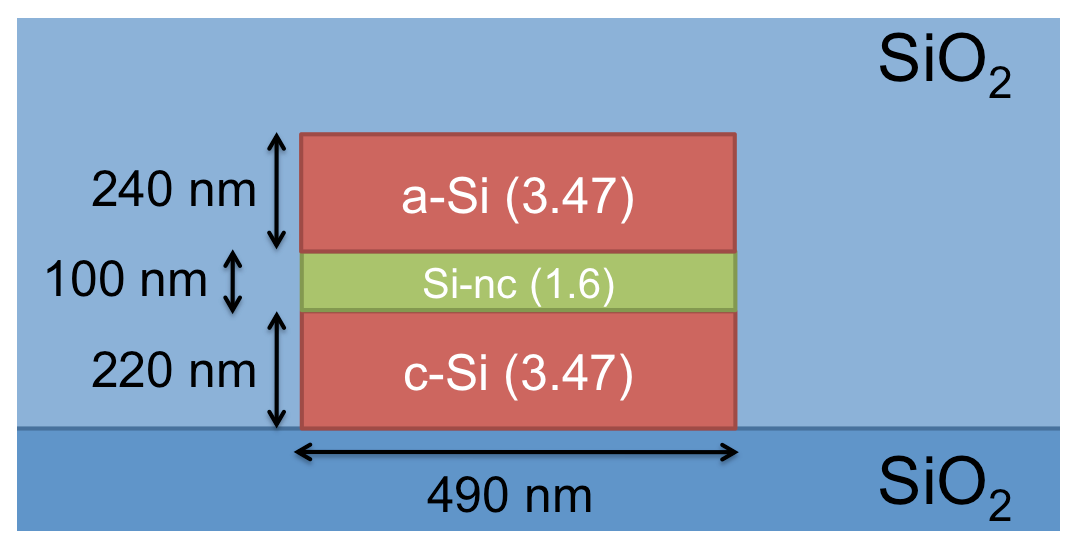
\includegraphics[width=0.42\textwidth]{slot5}%0.6
\caption{Silicon-nanocrystals (Si-nc) slot waveguide schema. Top made of amorphous silicon (a-Si) and bottom of crystalline silicon (c-Si).
Refractive index of the Si-nc layer was measured from a thick Si-nc sample using the m-lines technique.}
\label{fig:semSlot}
\end{figure}


\section{Nonlinear loss measurements: Im$ (\gamma) $}
\label{sec:imGammaTimeRes}
First, we characterized the nonlinear loss in all the samples under test.
Two-photon absorption (TPA) is a well-known process in silicon waveguides, and can be considered as the imaginary part of the gamma coefficient using the differential equation derived in \cite{Mizrahi}:

\begin{equation}
\frac{dP}{dz} = -\alpha P(z) - 2|Im(\gamma)| P(z)^2 
\label{eq:differentialTPAtimeRes}
\end{equation}

where $P$ is the signal power through the waveguide, $\alpha$ is the linear loss of the waveguide, and Im$(\gamma)$ is the imaginary part of the $\gamma$ coefficient (we use the absolute value because we want to stress its loss character in the equation with a negative sign). 
The solution of the differential equation shown in Eq.~\ref{eq:differentialTPAtimeRes} after a distance $L$ is given by:

\begin{equation}
P(L) = \frac{e^{-\alpha_0 L}}{1+2|Im(\gamma)| L_{eff} P_0} P_0
\end{equation}

where $P_0$ is the input power in the waveguide and $ L_{eff} $ the effective length:

\begin{equation}
L_{eff} = \frac{1-e^{-\alpha_0L}}{\alpha_0}
\end{equation}


Therefore the impact of nonlinear losses ($T_{NL}^{-1}$) on the overall transmission can be calculated as the ratio between the transmission at low power ($T_{LP} = e^{-\alpha_0 L} $) and the transmission at high power ($T_{HP} = P(L)/P_0 $). In particular the inverse of $T_{NL}$ turns out to be a linear function of $P_0$:

\begin{equation}
T_{NL}^{-1} = \frac{T_{LP}}{T_{HP}} = 1+2|Im(\gamma)| L_{eff} P_0
\label{eq:transmissionLinearTimeRes}
\end{equation}

As a consequence, if we plot this ratio as a function of $P_0$, the slope of the curve can give us the two-photon absorption coefficient of the waveguide as in~\cite{Vallaitis2009}.
However, this equation is only valid for instantaneous transmission values.
We find that when a pulsed signal $P_0(t)$ is launched into the waveguide, the measured transmission is time averaged, so defining $ \tilde{T} $ as the integrated transmission along the duration of the pulse, the equivalent nonlinear loss $\tilde{T}_{NL}^{-1}$ can be expressed as:

                                                                \begin{equation}
                                                                        \tilde{T}_{NL}^{-1} = \frac{\tilde{T}_{LP}}{\tilde{T}_{HP}} = \frac{\int P_0(t)dt}{\int \frac{P_0(t)}{1+2|Im(\gamma)| L_{eff} P_0(t)} dt}
                                                                        \label{eq:transmissionIntegralTimeRes}
                                                                \end{equation}

If the pulsed signal has a rectangular shape, one can use Eq.~\ref{eq:transmissionLinearTimeRes}, but if the shape is different, the integral in Eq.~\ref{eq:transmissionIntegralTimeRes} must be solved, as the result differs significantly.
The reason for this variation is the fact that the flanks of the pulse are not affected as hardly by TPA as the peak.
Therefore, the overall energy transmission is higher than for the case of cw excitation.
For the particular case of a $sech^2$ shape, which corresponds to the output of our laser, emitting 1-ps pulses with a repetition rate of 20~MHz and a central wavelength of 1539~ nm, the time dependent power can be expressed by:

\begin{equation}
P_0(t)=P_{0 peak} sech^2 \left(\frac{t}{\tau}\right)
\label{eq:sech2timeRes}
\end{equation}

and substituting Eq.~\ref{eq:sech2timeRes} in Eq.~\ref{eq:transmissionIntegralTimeRes} and solving the integral, one obtains:

                                                                \begin{equation}
                                                                        \tilde{T}_{NL}^{-1}  = \frac{\tilde{T}_{LP}}{\tilde{T}_{HP}} \bigg|_{sech^2~shape}  = \frac{\sqrt{\delta({\delta + 1})}}{\ln(\sqrt{\delta}+\sqrt{\delta+1})} ~~\mathrm{where}~~  \delta = 2|Im(\gamma)| L_{eff} P_{0 peak}
                                                                        \label{eq:transmissionHypSecantTimeRes}
                                                                \end{equation}


We measured the $\tilde{T}_{LP}$ and $\tilde{T}_{HP}$ parameters by putting a variable attenuator at the laser output and using a power-meter.
The experimental results are shown in Fig.~2, together with the fitting curves obtained using Eq.~\ref{eq:transmissionHypSecantTimeRes} in order to extract the Im$(\gamma)$ parameter shown in Table \ref{tab:resultsArticleSlot}. 
It is worth noting that the Im$(\gamma )$ of slot waveguides is much lower than that of TE strip waveguides.
This can be easily explained considering that in the slot structure the main part of the optical field is confined within the region containing silicon oxide doped with silicon nanocrystals, which have a band-gap higher than that of crystalline Silicon as theoretically and experimentally demonstrated by several authors in the past years~\cite{Buuren98, Bassani, Daldosso2009}.
The low value of Im$(\gamma)$ measured in TM strip waveguide is due to the fact that the mode largely extends in the $\mathrm{SiO_2}$ cladding.

\begin{figure}[htb]
    \centering
    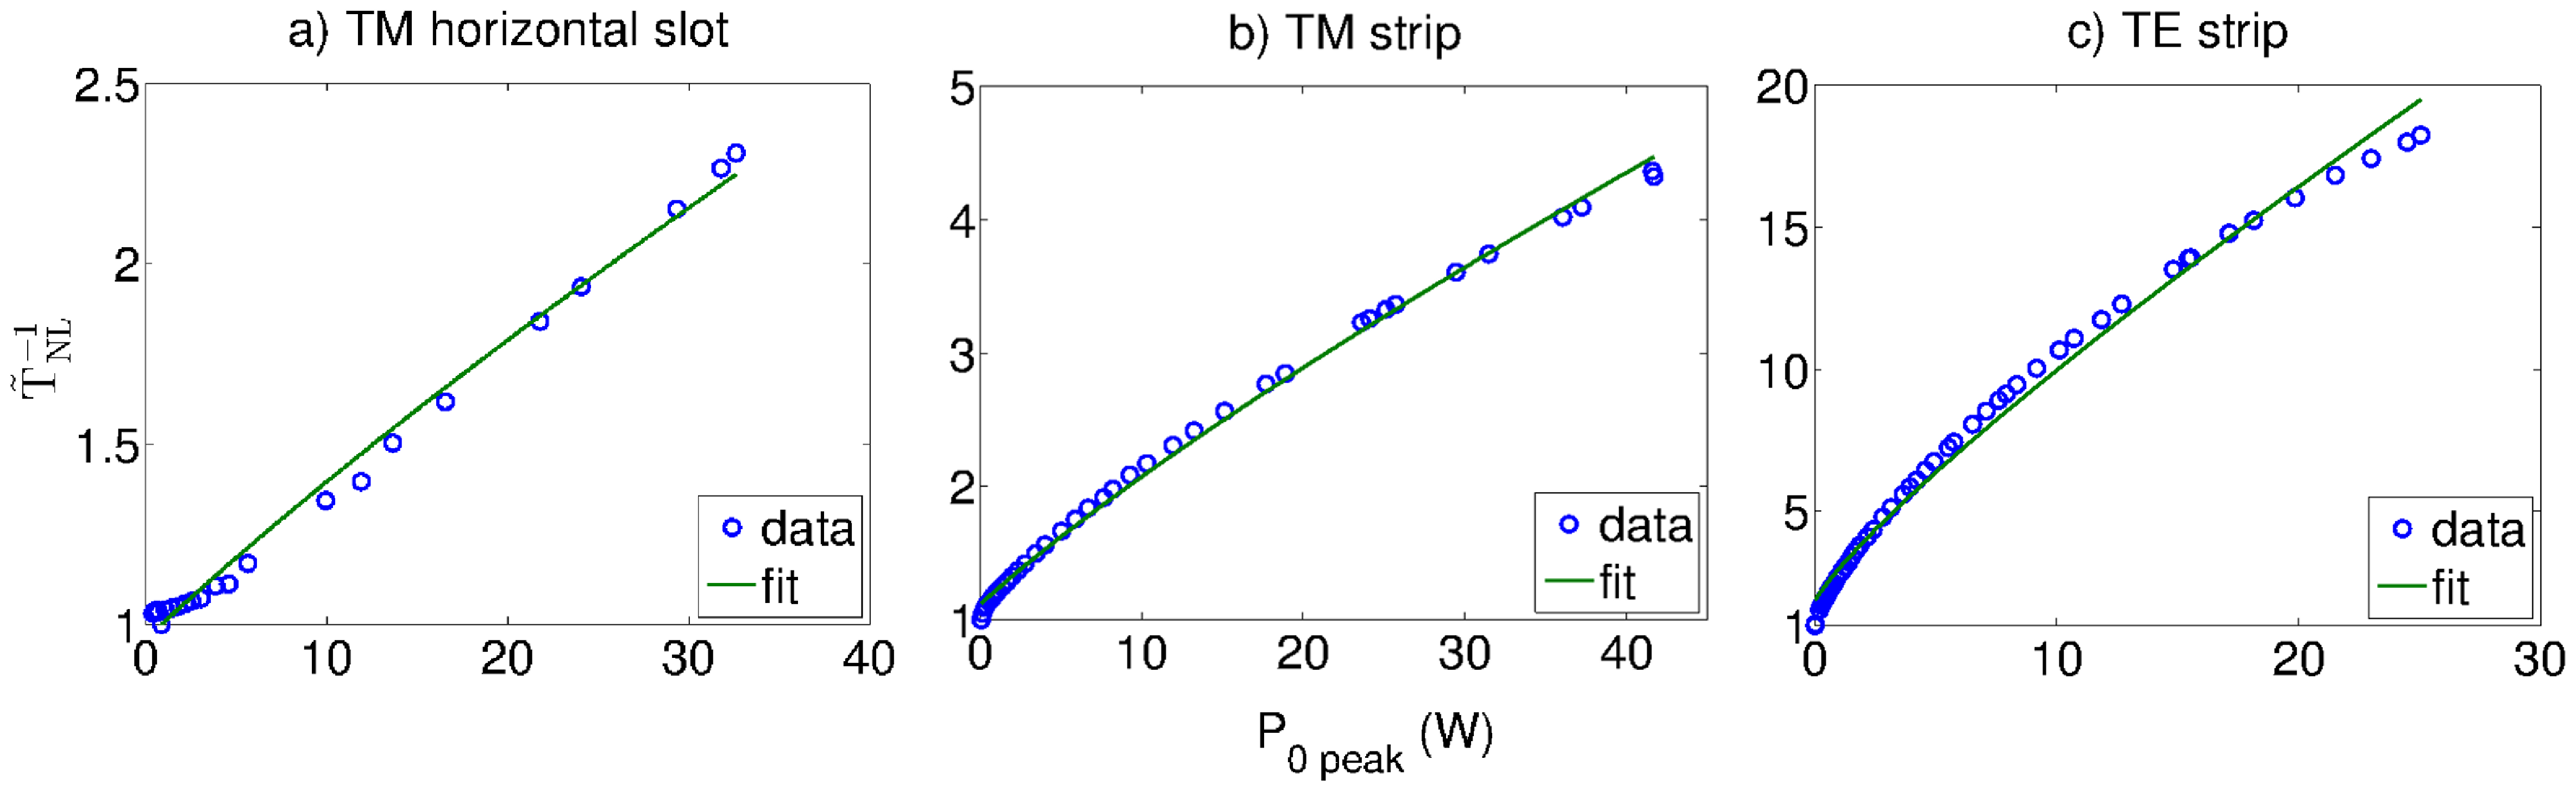
\includegraphics[width=1.0\textwidth]{imGamma_slot_TM_TE_v6}
     \caption{Transmission versus waveguide peak power (note the difference in the y-scale among the three plots). Solid line shows the fit for $ sech^2 $ pulses using Eq.~\ref{eq:transmissionHypSecantTimeRes}.}
    \label{fig:imGammaSamples}
\end{figure}



\section{Time-resolved measurements}
Time resolved measurements were performed in order to distinguish Kerr and TPA from carrier effects, using the technique described in \cite{Vallaitis2008}.
The set-up is shown in Fig.~\ref{fig:setupTimeResTimeRes}. We split the 1~ps pulse into three pulses: the most intense acts as a pump, while the two weaker pulses (reference and probe) are frequency shifted by two acousto-optic modulators (respectively by 80~MHz and 80.04~MHz ) and recombined with a fixed probe-to-reference delay of 10~ns.
All the pulses are then coupled inside the waveguide under test and the time-delay between probe pulse and pump pulse is changed by means of a variable delay line.
At the output, the probe and reference pulses are re-synchronized by a 10~ns delay-line and their beating signal is recovered by a lock-in amplifier.

                                \begin{figure}[htb]
                                         \centering
                                         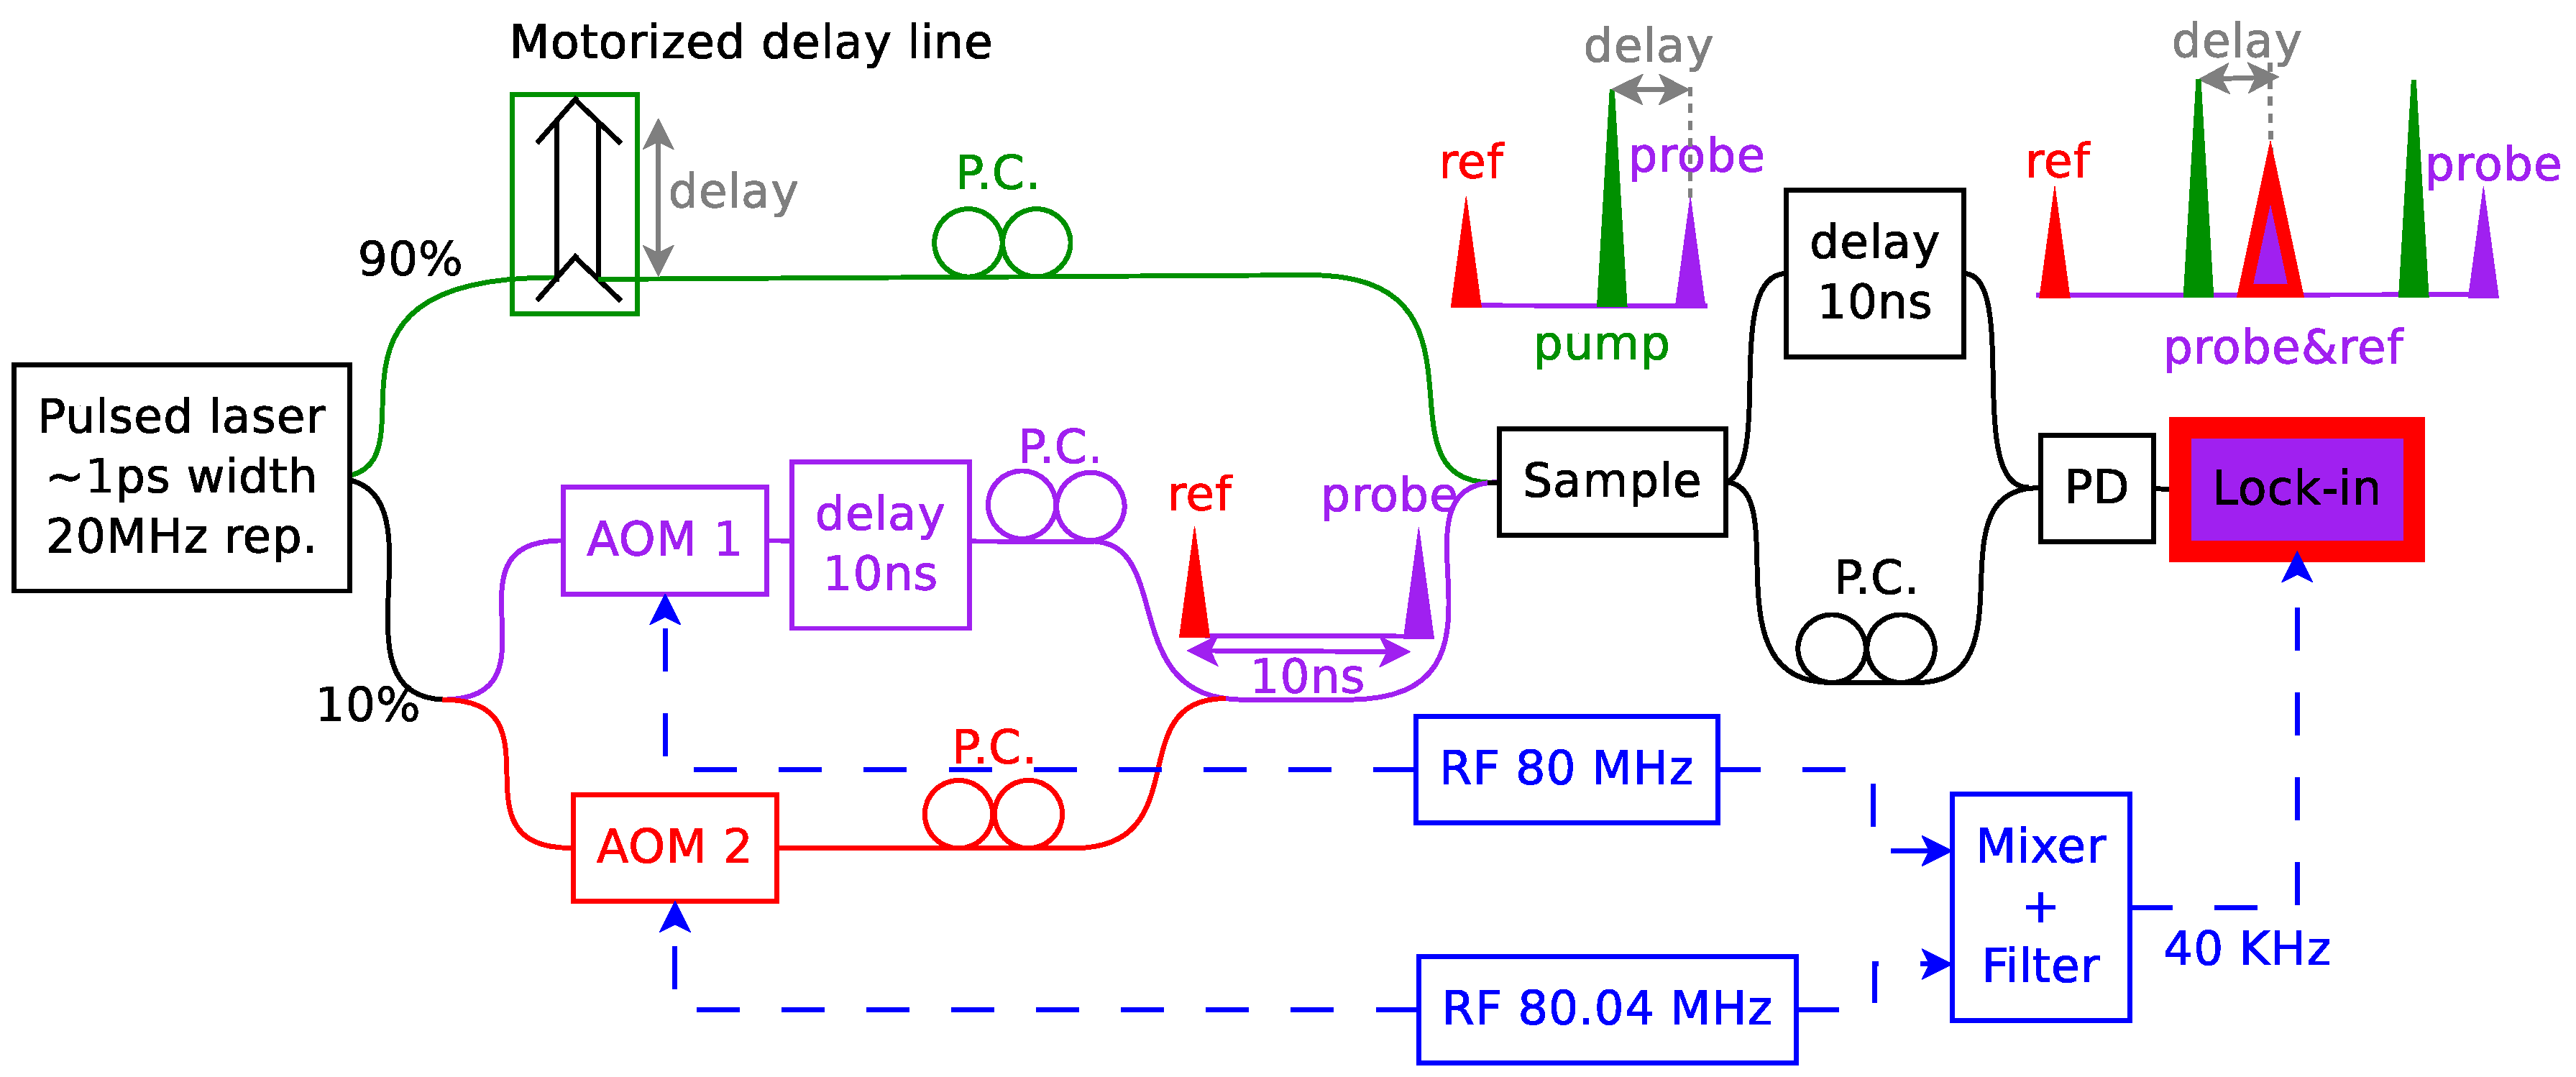
\includegraphics[width=0.95\textwidth]{timeResolved9}
                                         \caption{Time resolved characterization setup. PD: photodiode, PC: polarization controller, AOM: acousto-optic modulator.}
                                     \label{fig:setupTimeResTimeRes}
                                \end{figure}



In Fig.~\ref{fig:timeResolvesMeasurementsTimeRes} we observe the impact on transmission through the considered structures of both Kerr and carrier effect. The two effects produce opposite phase shifts because Kerr-effect increases the refractive index ($\Delta n > 0 $) and carriers decrease it ($ \Delta n < 0 $).  The dynamics  of these processes are also very different. During the pump pulse, an instantaneous phase change is due to Kerr effect; conversely after the pump pulse is gone, there is a phase response due to the carrier plasma effect (generally indicated as free-carrier dispersion - FCD) with positive sign that decays only on a much longer nanosecond time-scale. In order to investigate any degradation effects we exposed the waveguide to a high optical power for 1h and we did not observe any changes of the nonlinear optical performance.


\section{Time-resolved simulations}
In order to evaluate the propagation of pump and probe pulses in the optical waveguides and to fit Re$(\gamma)$ we applied the split-step simulation method to the nonlinear Schr\"{o}dinger equation (NLSE), considering the attenuation, dispersion, TPA, Kerr nonlinearity and the FCD effect.
Using this method the overall propagation-length is divided in a series of steps significantly smaller than both the pulse dispersive length and the nonlinear length ~\cite{Agrawal2001a,Lin2007}.
In the simulation program we inserted the experimentally measured waveguide losses, group velocity dispersion (measured using the technique reported in \cite{Mas2012}) and TPA coefficients obtained in section 3. Raman, pulse self-steepening, and higher-order dispersion terms terms have been neglected.
The effect of free carriers has been taken into account as in ~\cite{Lin2007}, where a carrier density averaged through the waveguide section is assigned to each simulation step. Carrier generation rate is governed by the TPA coefficient, while carrier decay time is assumed to be much longer than the pulse duration.
Finally the FCA and FCD coefficients dictate the effect of the carriers on the instantaneous absorption and refractive index of the waveguide respectively.
We have considered the FCA and FCD parameter definitions shown in Ref.~\cite{Lin2007}. In Table 1 we show all the parameters used in the simulation, except for the FCA coefficient, as from the experiment the effect of FCA was too weak to get a reliable estimation. By means of numerical simulations we obtain the envelope and the phase of the pump, probe and reference pulses at the waveguide output.
The output of the lock-in amplifier is the amplitude and the phase of the beatings produced by the heterodyne signal.
This magnitude is the Fourier component at 40~kHz of the sum of the reference and probe signals.
As the central frequencies of these two pulses differ in 40~kHz, this is equal to the overlap integral of their complex envelopes $E_{\mathrm{ref}}$ and $E_{\mathrm{probe}}$, obtaining:


                                                                \begin{equation}
                                                                        |T_{A}|e^{j\phi} =
                                                                        \frac{\int E_{\mathrm{ref}}(\tau) E^*_{\mathrm{probe}}(\tau) ~ \mathrm{d}\tau}
                                                                        {\int |E_{\mathrm{ref}}(\tau)|^2~\mathrm{d}\tau}
                                                                \end{equation}


 %\vspace*{-15pt}                                                                                                                          
                                                                
\begin{figure}[htb]
  \centering
  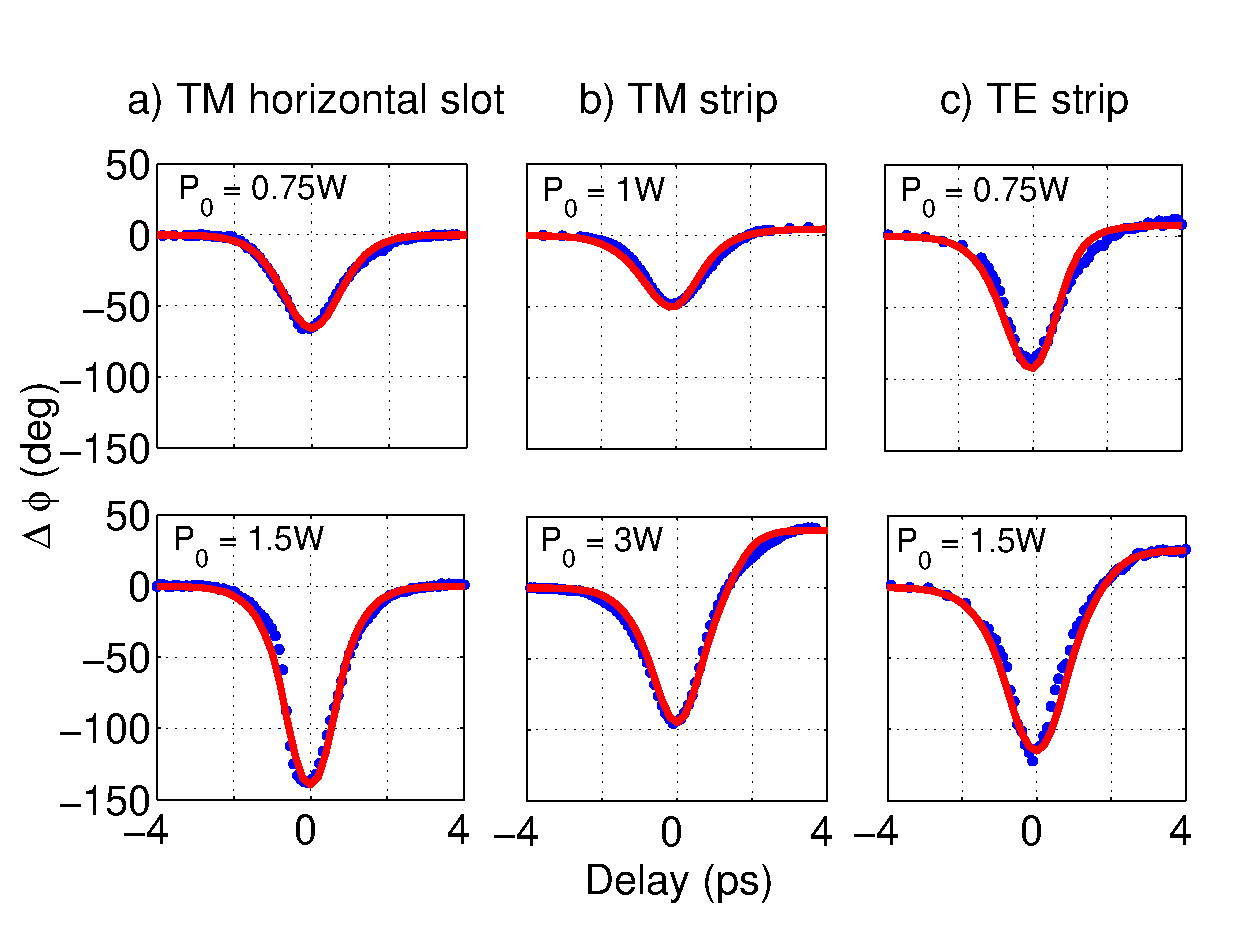
\includegraphics[width=0.77\textwidth]{measurements_v9}
  \caption{Time resolved measurements (blue dotted curves) and simulations (red continuous curves). Samples (a)TM-slot (0.75 and 1.5~W peak power) (b)TM-strip (1 and 3~W peak power) (c)TE-strip (0.75 and 1.5~W peak power).}
  \label{fig:timeResolvesMeasurementsTimeRes}
\end{figure}

where $T_A$ and $\phi$ are the amplitude and phase measured by the lock--in amplifier.
To evaluate Re$(\gamma)$ from the experimental data we performed numerical simulations (using a routine based on the split-step propagation method) in order to identify the Re$(\gamma)$ value yielding the best fit of the phase curve for each structure. In order to check for the results consistency we performed the experiments at two different power levels, obtaining two slightly different Re$(\gamma)$-values for each structure. In Table~\ref{tab:resultsArticleSlot} we report for each waveguide the average Re$(\gamma)$-value and its mean absolute deviation. 
The obtained results confirm that the slot-TM waveguide exhibits a higher nonlinear efficiency with respect to strip waveguides, that can be attributed to the high field confinement and to the interaction with silicon nanocrystals.


 \begin{table}[htb]
                        \centering
                        \caption{Extracted linear and nonlinear parameters from the experiment for the three samples: the horizontal slot, the  485$\times$220~nm TM strip and the  445$\times$220~nm TE strip waveguide. Dispersion values obtained with the technique shown in paper \cite{Mas2012}.}
                                \begin{tabular}{l|ccc}
                                        \hline
                                        Sample & TM slot & TM strip & TE strip\\\hline
                                        Coupling loss (dB) & 8 & 6 & 6\\
                                        Propagation loss (dB/cm) & 12 & 1.9 & 4.9\\
                                        $L_{eff}$ (mm) & 3.1 & 15.2 & 8.3\\
                                        Dispersion  (ps/(km$\cdot$nm))  & -1110 & -19800 & -1200\\
                                        $ Im(\gamma)~(\mathrm{W}\cdot \mathrm{m})^{-1} $          & -11.8 & -5.4 & -68.1\\
                                        $ Re(\gamma)~(\mathrm{W}\cdot \mathrm{m})^{-1} $          & 428$\pm$ 8 & 30 $\pm$ 3 & 235 $\pm$ 30\\
                                        $ FOM = \frac{1}{4\pi} \frac{Re(\gamma)}{|Im(\gamma)|} $  & 2.9 $\pm 0.06$ & 0.44 $\pm 0.05$ & 0.27$\pm 0.05$ \\
                                        effective FCD $ \frac{-\sigma_n}{ A_{eff} }~(10^{-15}~\mathrm{m}) $  & \textless 2 & 21 & 28 \\
                                        \hline
                                \end{tabular} 
\label{tab:resultsArticleSlot}
\end{table}



\section{Results and conclusion}
The first significant result is that phase measurements clearly show that the slot waveguide not only has a low TPA but also that free carriers have a negligible role.
This is clear from Fig. \ref{fig:timeResolvesMeasurementsTimeRes} where the phase-curve is only slightly affected by the free-carrier contribution. On the contrary the response of strip waveguides shows a long tail with $\Delta n <0$ for delay times longer than 1~ns.
This is confirmed by the FCD parameter, defined in~\cite{Lin2007} and shown in Table \ref{tab:resultsArticleSlot} (we have considered the effective FCD, which is normalized with the effective area, making it a device parameter like $\gamma$, rather than a material parameter).
This feature considerably reduces the undesired patterning effects when modulating a real bit pattern. On the other hand, the figure of merit (FOM) given by the ratio between Kerr effect and TPA is also significantly higher in the slot waveguide than in the strip waveguides: $2.9\pm 0.06$ for the slot, $0.44 \pm 0.05$ and $0.27 \pm 0.05$ respectively for the TM and TE strip waveguides, as reported in Table~\ref{tab:resultsArticleSlot}.
It is worth underlining that the FOM obtained by the TE and TM waveguides well agree with the values reported by state of the art all-silicon waveguides~\cite{Koos2007a}.


All these findings can be explained by the fact that in the slot waveguide, a considerable amount of energy travels through the slot layer, which provides a very efficient Kerr effect~\cite{Trita2011} and a weak TPA.
Nevertheless we note that the optical performance of such waveguides depends on their structure as well as on the conditions of deposition of both the silicon nanocrystals layer and the Si top layer. It is interesting to highlight that considering different waveguide diameters it is possible, according to~\cite{Rukhlenko2012}, to greatly reduce the effective area and increase the amount of energy traveling through the slot region in comparison to the current waveguide design.
That would allow increasing the beam intensity in the structure thus boosting the nonlinear effects, provided that the increase of coupling losses do not completely overtake the advantages given by the optimized structure.
On the other hand, comparing the TM and TE strips, we find that the TM has a higher FOM but lower $\gamma$ than the TE.
This is expected, as the TM mode is weakly confined in the vertical direction, therefore more energy travels through the cladding, which has lower Kerr coefficient and negligible TPA.
Finally, the performance of the device is similar to the one shown in Ref.~\cite{Vallaitis2008} for a polymer-filled vertical slot; however, our system, being made of inorganic materials and only requiring CMOS processes, is expected to provide more robust and stable devices with less temperature constraints. 

In conclusion, ultrafast nonlinear measurements show that silicon-nanocrystal-based horizontal slot waveguides show weaker carrier effects and better FOM than Si strip waveguides.
This makes the slot structure better suited for CMOS-compatible high-speed all-optical processing than simple Si strip waveguides.

\section*{Acknowledgments}
We acknowledge EU-project PHOLOGIC (FP6-IST-NMP-017158), Spanish Ministry of Science and Innovation SINADEC (TEC2008-06333) and PROMETEO/2010/087 NANOFOTONICA projects and Universidad Polit\'ecnica de Valencia for PAID2011/1914 and J. Matres' doctoral grant.


%\bibliographystyle{osajnl}
%\bibliography{library}
\bibliographystyle{unsrt}
\begin{thebibliography}{10}
\newcommand{\enquote}[1]{``#1''}

\bibitem{Almeida2004b}
V.~R. Almeida, C.~A. Barrios, R.~R. Panepucci, and M.~Lipson,
  \enquote{{All-optical control of light on a silicon chip.}} Nature
  \textbf{431}, 1081--1084 (2004).

\bibitem{Lee2009}
B.~G. Lee, A.~Biberman, A.~C. Turner-Foster, M.~A. Foster, M.~Lipson, A.~L.
  Gaeta, and K.~Bergman, \enquote{{Demonstration of broadband wavelength
  conversion at 40 Gb/s in silicon waveguides},} IEEE Photon. Technol. Lett. \textbf{21}, 182--184 (2009).

\bibitem{Driscoll2010}
J.~B. Driscoll, W.~Astar, X.~L.~X. Liu, J.~I. Dadap, W.~M.~J. Green, Y.~A.
  Vlasov, G.~M. Carter, and R.~M. Osgood, \enquote{{All-optical wavelength
  conversion of 10 Gb/s RZ-OOK data in a silicon nanowire via cross-phase
  modulation: Experiment and theoretical investigation},} IEEE J. Sel. Top. Quantum Electron \textbf{16}, 1448--1459 (2010).

\bibitem{Koos2009}
C.~Koos, P.~Vorreau, T.~Vallaitis, P.~Dumon, W.~Bogaerts, R.~Baets,
  B.~Esembeson, I.~Biaggio, T.~Michinobu, F.~Diederich, W.~Freude, and
  J.~Leuthold, \enquote{{All-optical high-speed signal processing with silicon
  – organic hybrid slot waveguides},} Nature Photonics \textbf{3}, 1--4
  (2009).

\bibitem{Astar2010}
W.~Astar, J.~B. Driscoll, X.~L.~X. Liu, J.~I. Dadap, W.~M.~J. Green, Y.~A.
  Vlasov, G.~M. Carter, and R.~M. Osgood, \enquote{{All-Optical Format
  Conversion of NRZ-OOK to RZ-OOK in a Silicon Nanowire Utilizing Either XPM or
  FWM and Resulting in a Receiver Sensitivity Gain of 2.5 dB},} IEEE J. Sel. Top. Quantum Electron \textbf{16}, 234--249 (2010).

\bibitem{Foster2008}
M.~A. Foster, A.~C. Turner, M.~Lipson, and A.~L. Gaeta, \enquote{{Nonlinear
  optics in photonic nanowires.}} Opt. Express \textbf{16}, 1300--1320
  (2008).

\bibitem{Osgood2009}
R.~M. Osgood, Jr., N.~C. Panoiu, J.~I. Dadap, X.~Liu, X.~Chen, I.-W. Hsieh,
  E.~Dulkeith, W.~M. Green, and Y.~A. Vlasov, \enquote{{Engineering
  nonlinearities in nanoscale optical systems: physics and applications in
  dispersion-engineered silicon nanophotonic wires},} Adv. Opt. Photon. \textbf{1}, 162 (2009).

\bibitem{Almeida2004}
V.~R. Almeida, Q.~Xu, C.~A. Barrios, and M.~Lipson, \enquote{{Guiding and
  confining light in void nanostructure.}} Opt. Lett. \textbf{29}, 1209--1211
  (2004).

\bibitem{Sanchis2007}
P.~Sanchis, J.~Blasco, A.~Martinez, and J.~Marti, \enquote{{Design of
  Silicon-Based Slot Waveguide Configurations for Optimum Nonlinear
  Performance},} J. Lightwave Technol. \textbf{25}, 1298--1305
  (2007).

\bibitem{Koos2007a}
C.~Koos, L.~Jacome, C.~Poulton, J.~Leuthold, and W.~Freude, \enquote{{Nonlinear
  silicon-on-insulator waveguides for all-optical signal processing.}} Opt. Express \textbf{15}, 5976--5990 (2007).

\bibitem{Zhang2010}
L.~Zhang, Y.~Yue, Y.~Xiao-Li, J.~Wang, R.~G. Beausoleil, and A.~E. Willner,
  \enquote{{Flat and low dispersion in highly nonlinear slot waveguides.}}
  Opt. Express \textbf{18}, 13187--13193 (2010).

\bibitem{Rukhlenko2012}
I.~D. Rukhlenko, M.~Premaratne, and G.~P. Agrawal, \enquote{{Effective mode
  area and its optimization in silicon-nanocrystal waveguides.}} Opt. Lett.
  \textbf{37}, 2295--2297 (2012).

\bibitem{Spano2009}
R.~Spano, N.~Daldosso, M.~Cazzanelli, L.~Ferraioli, L.~Tartara, J.~Yu,
  V.~Degiorgio, E.~Giordana, J.~M. Fedeli, and L.~Pavesi, \enquote{{Bound
  electronic and free carrier nonlinearities in Silicon nanocrystals at
  1550nm.}} Opt. Express \textbf{17}, 3941--3950 (2009).

\bibitem{Martinez2010a}
A.~Mart\'{\i}nez, J.~Blasco, P.~Sanchis, J.~V. Gal\'{a}n,
  J.~Garc\'{\i}a-Rup\'{e}rez, E.~Jordana, P.~Gautier, Y.~Lebour,
  S.~Hern\'{a}ndez, R.~Guider, N.~Daldosso, B.~Garrido, J.~M. Fedeli,
  L.~Pavesi, J.~Mart\'{\i}, and R.~Spano, \enquote{{Ultrafast all-optical
  switching in a silicon-nanocrystal-based silicon slot waveguide at telecom
  wavelengths.}} Nano Lett. \textbf{10}, 1506--1511 (2010).

\bibitem{Oton2010}
C.~J. Oton, J.~Matres, A.~Martinez, P.~Sanchis, J.~P. Colonna, C.~Ratin, J.~M.
  Fedeli, and J.~Marti, \enquote{{Ultrafast all-optical logic gates with
  silicon nanocrystal-based slot waveguides},} in Proc. of 7th IEEE Int. Conf. on Group IV Photonics, 171–-173 (IEEE, 2010).

\bibitem{Trita2011}
A.~Trita, C.~Lacava, P.~Minzioni, J.-P. Colonna, P.~Gautier, J.-M. Fedeli, and
  I.~Cristiani, \enquote{{Ultra-high four wave mixing efficiency in slot
  waveguides with silicon nanocrystals},} Appl. Phys. Lett. \textbf{99},
  191105 (2011).

\bibitem{Garcia2004}
C.~Garcia, B.~Garrido, P.~Pellegrino, J.~R. Morante, M.~Melchiorri,
  N.~Daldosso, L.~Pavesi, E.~Scheid, and G.~Sarrabayrouse, \enquote{{Low loss
  Silica waveguides containing Si nanocrystals},} in \enquote{New Materials for
  Microphotonics, Ed. J. H. Shin, M. Brongersma, C. Buchal, F. Priolo, MRS
  Proceedings,}  (2004),\textbf{817}, L4.1--L4.6.

\bibitem{Jordana2007}
E.~Jordana, J.-M. Fedeli, P.~Lyan, J.~P. Colonna, P.~E. Gautier, N.~Daldosso,
  L.~Pavesi, Y.~Lebour, P.~Pellegrino, B.~Garrido, J.~Blasco, F.~Cuesta-Soto,
  and P.~Sanchis, \enquote{{Deep-UV Lithography Fabrication of Slot Waveguides
  and Sandwiched Waveguides for Nonlinear Applications},} in Proc. of 4th IEEE Int. Conf. on Group IV Photonics, 1–-3 (IEEE, 2007).
  
\bibitem{Mizrahi}
V.~Mizrahi, K.~W. Delong, G.~I. Stegeman, M.~A. Saifi, and M.~J. Andrejco,
  \enquote{{Two-photon absorption as a limitation to all-optical switching.}}
  Opt. Letters \textbf{14}, 1140--1142 (1989).

\bibitem{Vallaitis2009}
T.~Vallaitis, S.~Bogatscher, L.~Alloatti, P.~Dumon, R.~Baets, M.~L. Scimeca,
  I.~Biaggio, F.~Diederich, C.~Koos, W.~Freude, and J.~Leuthold,
  \enquote{{Optical properties of highly nonlinear silicon-organic hybrid (SOH)
  waveguide geometries.}} Opt. Express \textbf{17}, 17357--17368 (2009).
  
\bibitem{Buuren98}
T.~van Buuren, L.~Dinh, L.~Chase, W.~Siekhaus, and L.~Terminello, \enquote{{Changes in the Electronic Properties of Si Nanocrystals as a Function of Particle Size}}. Phys. Rev. Lett., \textbf{80}, 3803–-3806 (1998).

\bibitem{Bassani}
Z.~Gaburro, N.~Daldosso, L.~Pavesi, \enquote{Porous Silicon}, Encyclopedia of Condensed Matter Physics edited by F.~ Bassani, J.~Liedl and P.~Wyder (Elsevier Academic Press, 2005)

\bibitem{Daldosso2009}
N.~Daldosso and L.~Pavesi, \enquote{Nanosilicon photonics}. Laser Photonics Rev., \textbf{3}, 508–-534 (2009).

\bibitem{Vallaitis2008}
T.~Vallaitis, C.~Koos, R.~Bonk, W.~Freude, M.~Laemmlin, C.~Meuer, D.~Bimberg,
  and J.~Leuthold, \enquote{{Slow and fast dynamics of gain and phase in a
  quantum dot semiconductor optical amplifier.}} Opt. Express \textbf{16},
  170--178 (2008).

\bibitem{Agrawal2001a}
G.~P. Agrawal, \emph{{Nonlinear Fiber Optics}}, (Academic Press, 2001).

\bibitem{Lin2007}
Q.~Lin, O.~J. Painter, and G.~P. Agrawal, \enquote{{Nonlinear optical phenomena
  in silicon waveguides: modeling and applications.}} Opt. Express
  \textbf{15}, 16604--16644 (2007).

\bibitem{Mas2012}
S.~Mas, J.~Matres, J.~Marti, and C.~J. Oton, \enquote{{Accurate chromatic
  dispersion characterization of photonic integrated circuits},} IEEE Photon. J. \textbf{4}, 825--831 (2012).

\end{thebibliography}
